
\chapter{The ATLAS Experiment at the Large Hadron Collider}
\label{chap:experiment}
Testing the theoretical predictions and models of high-energy physics in the 21st century requires huge experimental setups with unprecedented size and complexity.
The ATLAS experiment~\cite{PERF-2007-01} is one of the two general purpose detectors measuring the particle-particle collision events produced by the \emph{Large Hadron Collider} (LHC)~\cite{Evans:2008zzb} to an extreme precision. It is designed to measure a broad range of physics processes with a specific focus on observing and measuring the Higgs boson.
The LHC is the most powerful particle accelerator to date. It remains the most recent large-scale upgrade to the accelerator complex at CERN, the European Organization for Nuclear Research, and produces collision events at unprecedented energies.
This chapter provides an overview of the LHC, followed by a detailed description of the ATLAS detector and its various subcomponents.

\Minote{}{Mention previous experiments? Tevatron, ...other?}

\section{The Large Hadron Collider}
To produce collision events at the highest energies, circular accelerators are built in order to increase the particles' energy step-wise. The two major technical components are \emph{radiofrequency cavities} (RF cavities) with oscillating electromagnetic field to accelerate the particles as well as organizing them in so-called \emph{bunches}\footnote{RF cavities oscillate at a given frequency. Particles arriving early (late), will be decelerated (accelerated) so that the particles are kept together in discrete packages called bunches.} and magnet systems to bend, steer, and focus the particles' trajectories. The peak particle energy reached by a hadron collider is thereby limited by the maximum field strength reached by the bending magnets.

The LHC was designed and built for more than two decades starting in the early 1980s by more than $10000$ international researchers, engineers, and technicians from more than $100$ different countries.
The LHC is placed in a near-circular tunnel\footnote{The same tunnel was used by the former LEP collider~\cite{LEPDesignReport}.} \SI{100}{\m} underground below the France-Switzerland border close to Geneva (Switzerland). It has a circumference of \SI{26.7}{\km} and collides protons in its main mode of operation\footnote{The LHC also produces heavy-ion collisions in dedicated running periods}. Proton bunches are accelerated with 16 RF cavities oscillating at \SI{400}{\mega\hertz} in two close-by rings to form counter-rotating beams. During operation, the LHC allows to contain a maximum of 2808 bunches separated by a bunch spacing of \SI{25}{\ns} and with about \SI{e11}{protons} in each bunch, which results in a design instantaneous luminosity of $\mathcal{L} = \SI{e34}{\per\cm\per\s}$.\footnote{The machine and beam parameters of the LHC can vary between different data-taking cycles. More details can be found in \cref{sec:run-2-data-taking}.}
More than 1200 superconducting twin-bore dipole magnets are used to force the particle beams on a curved trajectory.
They are designed to reach field strengths of up to \SI{8.33}{\tesla}, leading to a design centre-of-mass energy of $\sqrt{s} = \SI{14}{\TeV}$. More than 400 quadrupole magnets are used to ``squeeze'' the beams to increase the particle density within each bunch, which is especially important before the beams are made to collide at one of the four main \emph{interaction points} (IP). Each IP is surrounded by large detector systems that are optimized and designed to measure different physics processes as precisely as possible.
The ATLAS and CMS~\cite{CMS-TDR-08-001} experiments are general purpose detectors, designed to measure a large variety of physics processes; the LHCb\footnote{Large Hadron Collider beauty} experiment~\cite{1748-0221-3-08-S08005} is dedicated to measuring processes that involve $b$-quarks; and ALICE\footnote{A Large Ion Collider Experiment}~\cite{1748-0221-3-08-S08002} focuses on the analysis of heavy-ion collisions.\footnote{There are other smaller experiments operating at the LHC: the TOTEMd (Total Elastic and Diffractive Cross Section Measurement)~\cite{1748-0221-3-08-S08007} and LHCf (Large Hadron Collider forward)~\cite{1748-0221-3-08-S08006} experiments study scattering processes close to the beam line and the MoEDAL (Monopole and Exotics Detector at the LHC) experiment~\cite{1742-6596-631-1-012014} is dedicated to the search for magnetic monopols.}

In so-called \RunOne of the LHC, that took place between 2011 and 2012, protons were collided at $\sqrt{s} = 7\,\TeV$ and $\sqrt{s} = 8\,\TeV$, respectively. \RunTwo of the LHC refers to the data-taking period between 2015 and 2018 and delivered collisions at $\sqrt{s} = \SI{13}{\TeV}$. After a technical shutdown between 2018 and 2022, the LHC is expected to continue to operate with \RunThr at a centre-of-mass energy of at least $\sqrt{s} = \SI{13}{\TeV}$\footnote{At the time of writing, the details of the \RunThr running conditions had not yet been determined}.\Rnote{}{Any news on the actual energy that will be used?}
The data recorded by the ATLAS experiment in \RunTwo is analyzed throughout this thesis. Further details on the \RunTwo data taking are given in \cref{sec:run-2-data-taking}.


\subsection{The accelerator complex}
Before the protons enter the LHC, they pass through a sophisticated chain of smaller accelerators. A schematic of the entire accelerator complex is depicted in \cref{fig:accelerator-complex}.
The protons are extracted by ionizing hydrogen atoms and first accelerated in the linear accelerator \emph{Linac2} (Linear accelerator 2)\footnote{Starting in 2020, Linac2 will be replaced by a new linear accelerator, Linac4 (Linear accelerator 4). More information can be found in \ccite{CERN-AB-2006-084}.}. Three synchrotrons follow, which have an increasingly larger circumference and gradually increase the energy of the proton beams: The \emph{BOOSTER} (Proton Synchrotron Booster), the \emph{PS} (Proton Synchrotron), and the \emph{SPS} (Super Proton Synchrotron). The proton beams in the SPS reach an energy of $450\,\GeV$ and are then injected into the LHC. The whole ramp-up phase until stable beams at their final energies are brought to collision takes around 45 minutes. The LHC experiments then record the collision events for ideally about 8-10 hours or more until the intensity of the beams becomes too low, making it more efficient to dump the beam and start a new cycle.

\begin{figure}
    %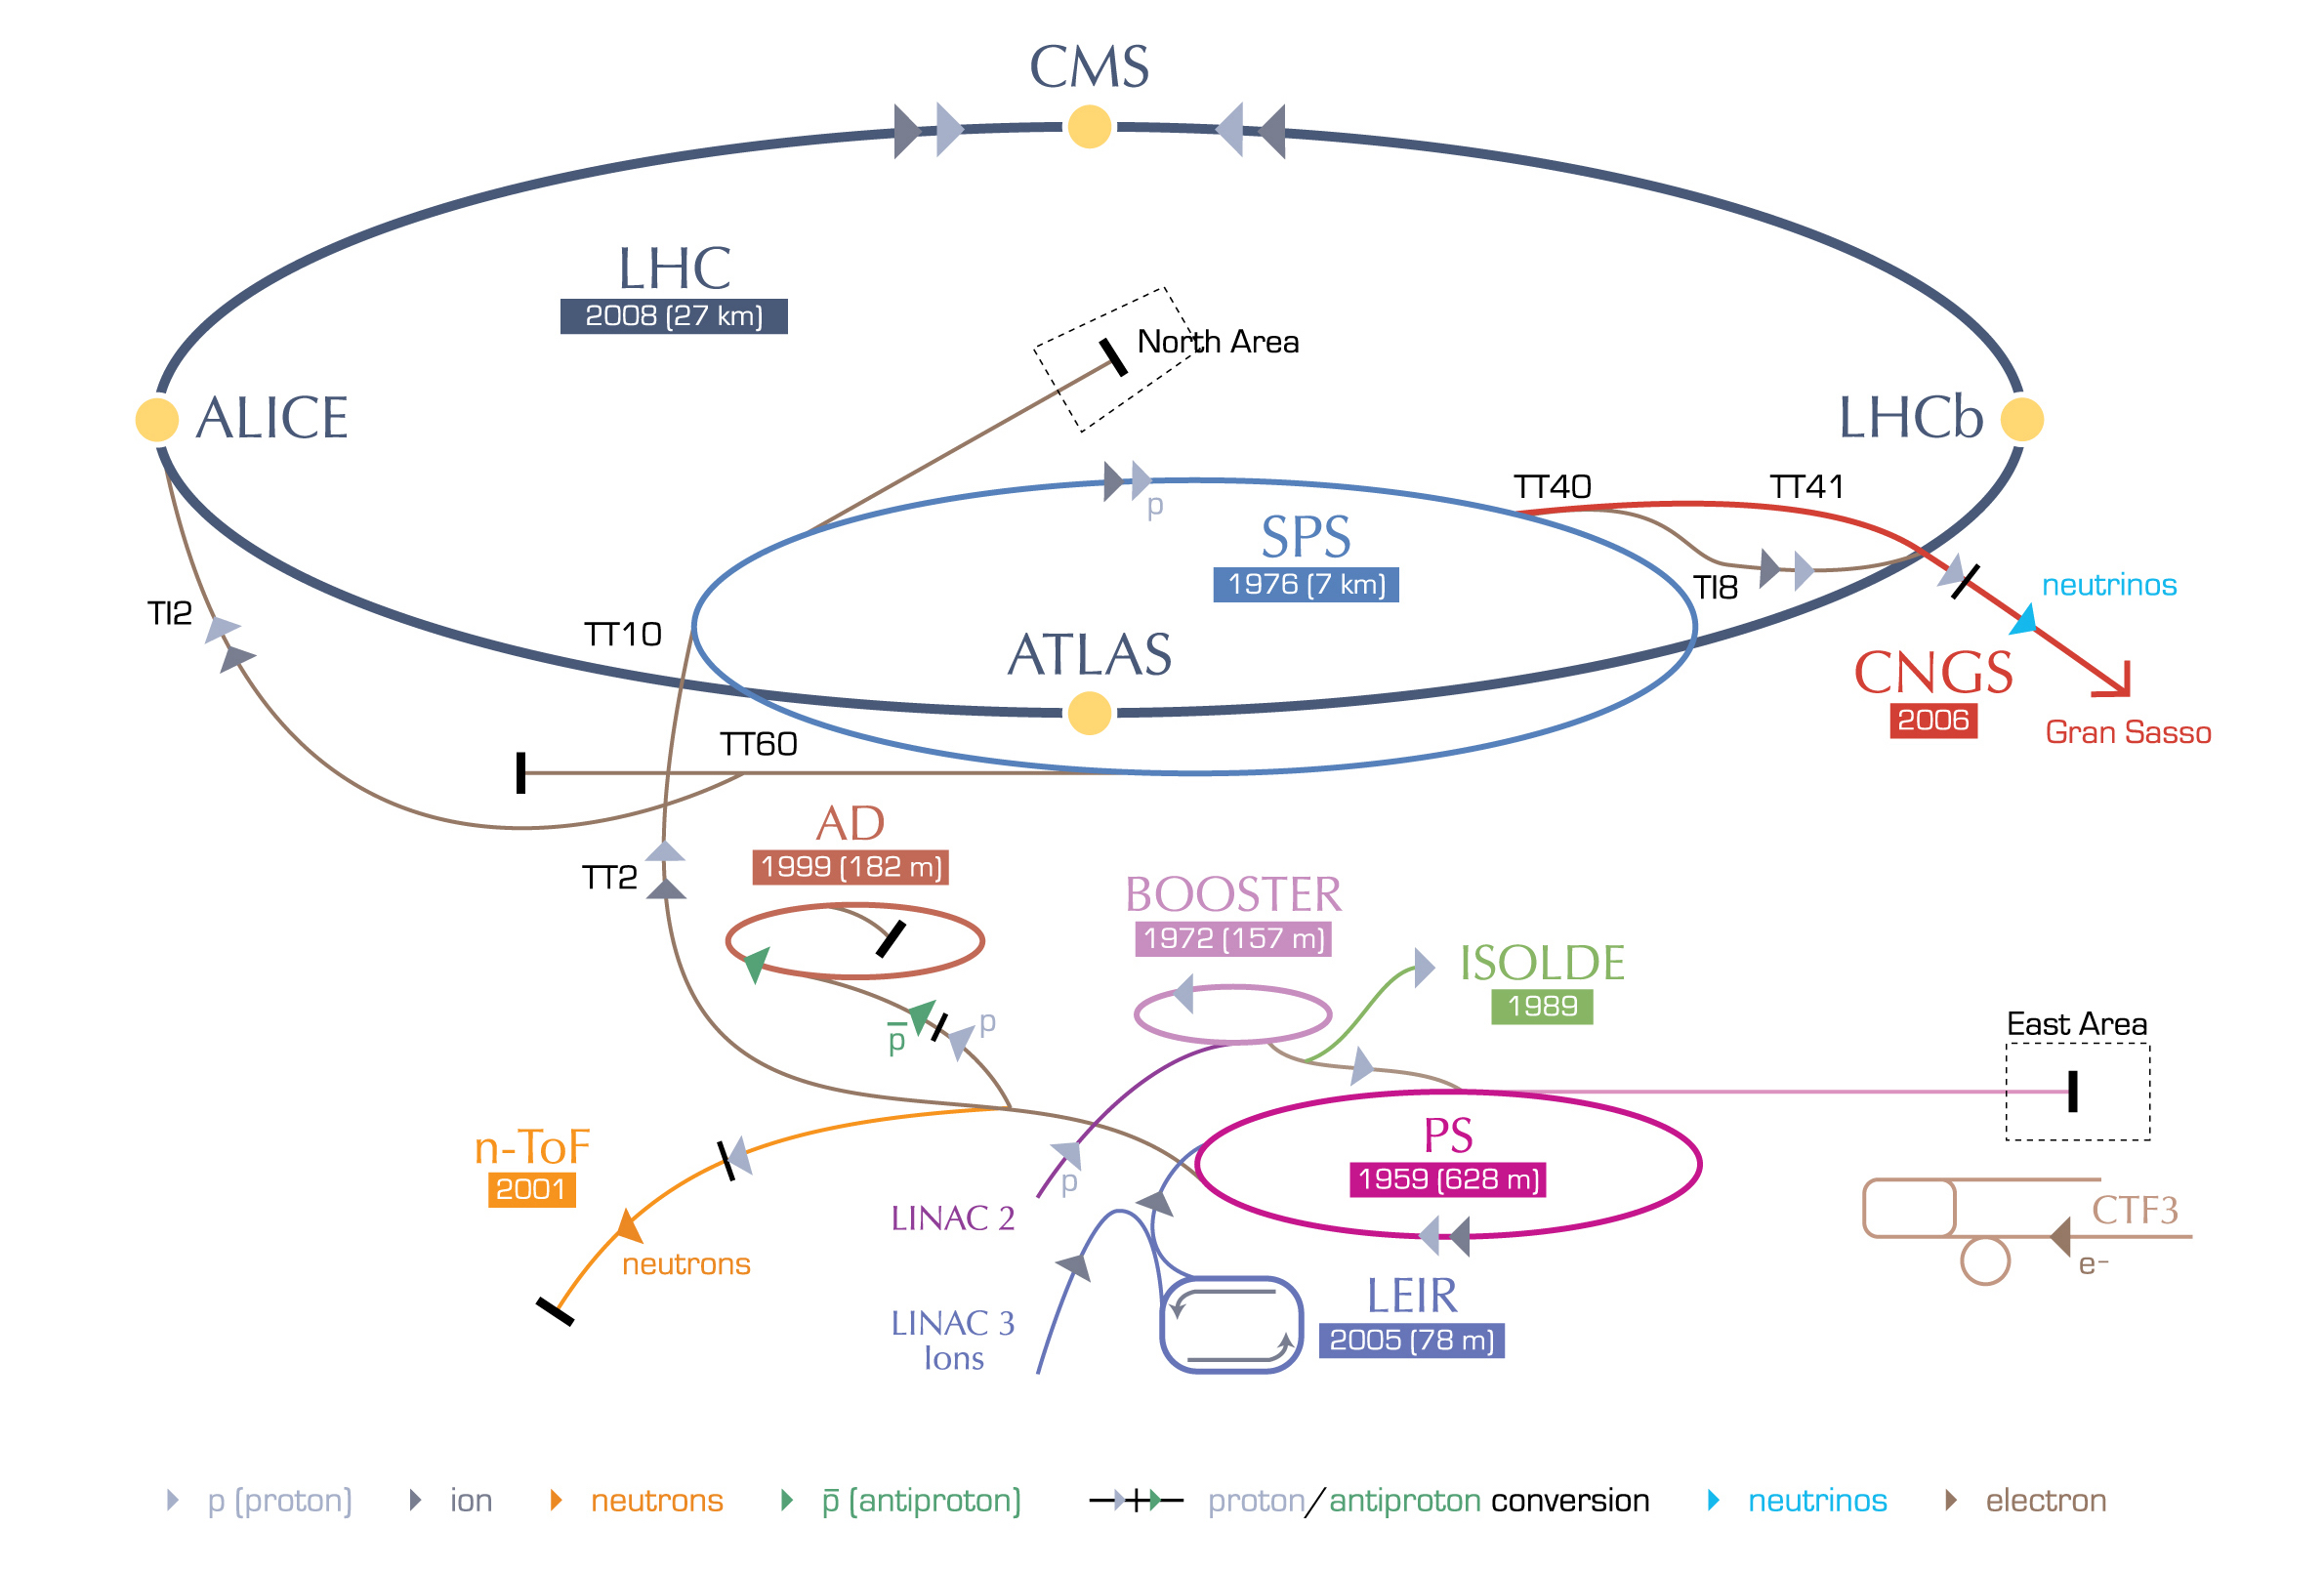
\includegraphics{figures/experiment/accelerator-complex.jpg}
    \newImageResize{figures/experiment/accelerator-complex.jpg}
    \caption[Schematic of the ATLAS detector showing the various subsystems.]{Schematic of the ATLAS detector showing the various subsystems. Adapted from \ccite{Christiane:1260465}.}
    \label{fig:accelerator-complex}
\end{figure}









\section{The ATLAS Experiment}

The ATLAS experiment is operated by one of the world's largest scientific collaborations. A community of about 3000 scientific authors from 181 institutions and 41 countries~\cite{AtlasCollab} work towards making the most precise measurements of the Standard Model and potentially finding experimental hints for New Physics with the ATLAS detector.
An illustration of the experiment is shown in \cref{fig:ATLASlayout}.
The ATLAS detector is \SI{44}{\meter} long and \SI{25}{\meter} high and has a forward-backward symmetric geometry covering almost $4\pi$ in solid angle.

Several layers are arranged in a cylindrical structure around the beam axis.
The different layers serve different functions and complement each other to form a detector system that is able to measure a wide range of physics processes.
The innermost layer, the \emph{inner detector} (ID), serves as a tracking device for charged particle trajectories. It is surrounded by a solenoid magnet that forces the charged particles on a curved path that can be used to measure their momenta.
A large \emph{calorimeter system} is placed outside the solenoid and stops almost all electromagnetic and hadronically interacting particles to provide energy measurements. The outermost part is the \emph{muon spectrometer} (MS) that detects muon tracks. A large toroidal magnet system is placed in between the muon detectors to allow the measurement of muon momenta.

The following describes the design and functionality of the different components, starting with a description of the tracking devices, the ID and the MS, followed details on the calorimeter system.
A combination of these subsystems is also used to trigger on interesting physics events which is discussed thereafter.
This section concludes with a description of the ATLAS simulation infrastructure. 
While most of these sections are kept very brief, more details are provided on the calorimeter system, as it is the crucial component for the calibration measurement presented in the subsequent \cref{chap:calibration} of this thesis, describing the noise term measurements of the jet energy resolution.
Many more details about the ATLAS detector can be found in \ccite{PERF-2007-01}, which this chapter heavily relies on.


\begin{figure}
    \newImageResize{figures/experiment/ATLASdetector.jpg}
    \caption[Schematic of the ATLAS detector showing the various subsystems.]{Schematic of the ATLAS detector showing the various subsystems. Taken from \ccite{PERF-2007-01}.}
    \label{fig:ATLASlayout}
\end{figure}

\subsection{The ATLAS coordinate system}
A right-handed cartesian coordinate system is used to describe the hard scatter processes. The nominal interaction point is taken as the origin. The $z$-axis defines the beam direction, the $y$-axis points upwards, and the $x$-axis points to the centre of the LHC. The azimuthal angle $\phi$ is measured against the $x$-axis in the $x$-$y$ plane and the polar angle $\theta$ is the angle taken from the beam axis. 
The transverse component of the energy, \ET, or momentum, \pT, of a particle is a useful quantity to measure at collider experiments and is determined by the projection of the total energy or momentum onto the $x$-$y$ plane.
The position of a particle in the $z$-$y$ plane is typically described with the \emph{pseudorapidity} $\eta$, defined as\footnote{For massive objects the \emph{rapidity} $y = \frac{1}{2} \text{ln} \left( \frac{E + p_Z }{E-p_z} \right)$ is used, where $E$ is the energy and $p_z$ the momentum in $z$-direction. The rapidity is approximated by the pseudorapidity for $m \ll E$, which is typically the case in high-energy scattering events.}
\begin{equation}
    \eta = - \text{ln} \left( \tan \left( \frac{\theta}{2} \right) \right).
\end{equation}
This allows for an angular distance measurement $\Delta R$ between particles,
\begin{equation}
    \Delta R = \sqrt{ \left( \Delta \eta \right) ^2 + \left( \Delta \phi \right) ^2 },
\end{equation}
that is invariant under Lorentz transformations along the $z$-axis. 


\subsection{Tracking}
- Some general blah blah on tracking devices!
-> See Schouten's thesis


\subsection{The Inner Detector}
\label{subsec:inner-detector}
The ID enables the reconstruction of charged-particle tracks stemming from the hard scatter by recognizing patterns in the detected particle positions often referred to as \emph{hits}. The tracks are used for impact parameter determination, primary and secondary vertexing, as well as momentum measurements. The latter is made possible by the particles' curved trajectory within a magnetic field.
Charged particle hits are detected by layers of different silicon-based semiconductor detectors as well as gaseous ionization tubes.

A schematic view of the ID is shown in \cref{fig:ATLASinnerdetector}.
In the barrel region the tracking detectors are arranged in cylinders around the beam axis, while in the end-cap regions, the different layers are placed on disks perpendicular to the beam axis.
The ID covers a range \absetaST{2.5} and is immersed in a \SI{2}{\tesla} magnetic field that is provided by a \SI{5.8}{\m} long solenoid magnet.
The four innermost layers consist of \emph{silicon pixel} detectors that typically provide four space points for each charged particle. The first layer, the insertable $b$-layer~\cite{ATLAS-TDR-19,PIX-2018-001}, was installed before \RunTwo and is especially important for the reconstruction of the interaction vertices.
Four double layers of \emph{silicon-microstrip} detectors in the barrel and each end-cap region are arranged at an angle of \SI{40}{\milli\radian} relative to each other to provide additional four space points. 
The fine granularity of the pixel and microstrip sensors provide high-precision measurements of particle hits with intrinsic resolutions in $R$-$\phi \times z$ of $10 \times 115\,\mu\text{m}$ and $17 \times 580\,\mu\text{m}$, respectively.
The \emph{Transition Radiation Tracker} (TRT) consists of a large number of straw tubes filled with xenon-based gas that provide on average 36 additional hits at longer track lengths. The TRT covers a range \absetaST{2.0} and provides information in only the $R$-$\phi$ plane with a resolution of \SI{130}{\micro\meter}.
Apart from the position measurement, the TRT also generates and detects the amount of transition radiation produced by charged particles, which helps to differentiate electrons from charged pions.
%Apart from the position measurement, the TRT is sensitive to the Lorentz factor of charged particles, by measuring the amount of transition radiation. In combination with a momentum measurement this provides the ability to compute the mass of particles and thus, gives additional information to differentiate electrons from charged pions.

\begin{figure}
    %\resizebox{\textwidth}{!}{
    \subfloat[central region]{
        \newImageScale{figures/experiment/ATLASinnerdetector.pdf}{.105}
    }
    \subfloat[end-cap region]{
        \newImageScale{figures/experiment/ATLASinnerdetectorendcap.png}{.095}
    }
    %   }
    \caption{Schematic of the ATLAS inner detector in the (a) central region and (b) the end-cap region. The illustration for the end-cap region does not include the IBL, as it was taken from an older reference. Taken from Refs.~\cite{ATL-PHYS-PUB-2015-009} and~\cite{PERF-2007-01}, respectively.}
    \label{fig:ATLASinnerdetector}
\end{figure}


\subsection{The Muon Spectrometer}
Muons are minimum-ionizing and escape the calorimeter system. 
Therefore, a large MS forms the outermost part of the ATLAS detector. 
The MS serves two main purposes: measuring track hits for muon reconstruction as well as providing fast information to the trigger system.
\Cref{fig:ATLASmuonspectrometer} shows the MS with its large superconducting toroid magnets in between of several chambers that detect the muon's ionization energy.
The 8 barrel toroid magnets and 16 end-cap magnets cover the range \absetaST{1.4} and \absetaBT{1.6}{2.7}, respectively. They provide magnetic bending power of \numrange{0.5}{1}\,T to measure the muons' momenta. Precision-tracking chambers operate with an argon-based mixture and are arranged in three layers in both the barrel and end-cap regions. They cover a range \absetaST{2.7} and mostly consist of \emph{Monitored Drift Tubes}, that provide six to eight $\eta$ measurements. Only the innermost layer in the region \absetaBT{2}{2.7} is made out of multiwire proportional chambers called \emph{Cathode Strip Chambers} that are more resistant against radiation damage. They provide four space points in the $\eta$-$\phi$ plane. The detector chambers with fast readouts consist of \emph{Resistive Plate Chambers} (RPC) in the central-region within \absetaST{1.05} and \emph{Thin Gap Chambers} in the end-cap regions at \absetaBT{1.05}{2.4}. 
Their main purpose is to provide fast information to the L1 trigger system (discussed below in \cref{sec:trigger-system}), but also provide information complementary to the precision trackers to allow for a three-dimensional track reconstruction of the muon candidates.

% They provide information about traversing muons to the L1 trigger system that is discussed below within \numrange{15}{25}\,ns.
%The RPCs are gaseous parallel electrode-plates without a wire and 


\begin{figure}
    \newImageScale{figures/experiment/ATLASmuondetector.png}{.15}
    \caption{Schematic of the ATLAS muon spectrometer. Taken from \ccite{PERF-2007-01}.}
    \label{fig:ATLASmuonspectrometer}
\end{figure}


\subsection{Calorimetry}
The goal of the ATLAS calorimeter system is to measure and contain electromagnetic as well as hadronic showers in order to identify and measure electrons and photons as well as jets and missing transverse energy. A schematic view is shown in \cref{fig:ATLAScalorimeters}.
The calorimeters can be roughly divided into a very granular \emph{electromagnetic calorimeter} (ECAL), that targets electromagnetic showers, and a \emph{hadronic calorimeter}, which is thicker and provides the stopping power needed to measure and contain hadronic activity.\TDinote{}{I think I should align the wording to the schmeatic that is shown, i.e. EMEC, Tile barrel, Tile extended barrel, HEC, ....} Both systems consist of so-called \emph{sampling calorimeters} that are composed of alternating layers of active material, to measure the ionization energy of traversing particles, and highly-dense absorbers, to initiate the showering and stop the particles. 
They cover a large angle of \absetaST{4.9} and almost entirely limit the level of punch-through to the muon system to the irreducible level of muons and neutrinos. The different subsystems are discussed in more details below, beginning with the ECAL, followed by the hadronic systems, and concluding with a description of the \emph{Forward Calorimeter} (FCAL). The most important parameters related to the detector coverage and granularity are given in \cref{tab:ATLAScalorimeter-parameters}.

%total radiation lengths to limit punch-through into the muon system is 9.7 lambda and > 22 Xo for eta = 0.

\subsubsection{The Electromagnetic Calorimeter}
The ECAL consists of lead absorbers that are filled with \emph{liquid argon} (LAr) as active material using Kapton electrodes for readout.
It is arranged in an accordion-shaped structure to ensure full coverage in $\phi$.
The ECAL is subdivided into a barrel part covering \absetaST{1.475} and two end-caps - one on each side of the detector - in the range \absetaBT{1.375}{3.2}.

The barrel consists of two identical segments along the $z$-axis with a small gap of \SI{4}{\milli\meter} in between at $z=0$. A schematic of one of the barrel modules is shown in \cref{fig:ECALbarrel-module}. Each module is segmented in three layers in depth with varying granularity. The first layer provides high resolution in $\Delta \eta$ with cell sizes of only $0.025 / 8 \times 0.1$ in $\Delta \eta \times \Delta \phi$. This provides essential inputs for photon and pion identification. The second layer measures the bulk of the electromagnetic showers and is finer in $\Delta \phi$ with a cell sizes of $0.025 \times 0.025$ in $\Delta \eta \times \Delta \phi$. The third and coarsest layer in $\Delta \eta$ is designed to measuring the broad tail of the electromagnetic showers.
Together, the three segments provide a stopping power of 24 radiation lengths ($X_0$) and due to the high granularity also provide valuable space point measurements in addition to the data from the ID.

% - Accordion-shaped sampling detector (to provide full coverage in eta) with lead as absorber and LAr as active material.
% - EM cal with barrel in eta < 1.475 and end-cap 1.375 < eta < 3.2. 
% - Barrel has small gap of (4 mm) at z = 0. 
% - barrel module Shown in Figure. Three layers with varying granularity very useful for additional position measurement.
In the transition region between barrel and end-caps (\absetaBT{1.37}{1.52}), also known as ``crack'', a lot of material amounting to several $X_0$ lies in front of the calorimeter, which renders photon and electron identification difficult.
The end-caps consist of wheels placed on each side of the barrel.
They are composed of three layers in depth for the range \absetaST{2.5} and two layers for \absetaBT{2.5}{3.2} with varying thickness of the lead absorber. Details on the readout granularity is shown in \cref{tab:ATLAScalorimeter-parameters}.

To account for the energy that particles loose upstream of the ECAL, when traversing the ID and solenoid magnet, a presampler consisting of a thin LAr layer is used in the range \absetaST{1.8}.

% - end-caps are two wheels. 
% - Transition region between barrel and endcap known as "crack", rendering photon and electron identification difficult. 
% - "lead thickness optimized has three segments in eta < 2.5 and two section in depth for eta > 2.5."
% - Presampler: "to correct for energy lost by electrons and photons upstream of the calorimeter for eta < 1.8 presampler detector consisting of a thin LAr layer of 1.1cm (0.5cm) thickness in barrel (end-cap)."
% "correct energy losses due to material in inner detector."
% "account for energy lost by electrons and photons traversing the ID and solenoid"
% - high-resolution measurement of electrons, photons.

\subsubsection{The Hadronic Calorimeter}
The hadronic calorimeter can be subdivided into the \emph{Hadronic Tile} calorimeter and the \emph{Hadronic End-Cap Calorimeter} (HEC). They provide a stopping power of around 7-10 interaction lengths depending on the $\eta$ region. The granularity is much coarser than that of the ECAL which is shown in \cref{tab:ATLAScalorimeter-parameters}.

The Hadronic Tile calorimeter surrounds the barrel of the ECAL and uses steel as absorber with scintillator tiles in between. A single module is shown in \cref{fig:ATLASmodules-b}. The scintillating light induced by traversing particles is collected at photomultipliers mounted on the tile edges via wavelength-shifting fibers. This allows for almost perfect $\phi$ coverage. The large barrel extends to \absetaST{1.0} and is in between two \emph{extended barrels} covering the range \absetaBT{0.8}{1.7}. 

The HCAL uses copper as absorbing material and LAr as the active layer. One end-cap wheel on either side of the detector provides a coverage of \absetaBT{1.5}{3.2} and is segmented into two layers in depth.

\subsubsection{Forward Calorimeter}
At very large angles (\absetaBT{3.1}{4.9}) the calorimeter needs to be especially resistant against radiation. The FCAL consists of thick absorber layers, the first one of which is made out of copper and targets measurements of electromagnetic showers. Two more absorber layers using tungsten as material provide necessary stopping power (10 interaction lengths) for hadrons. LAr is used as active material between the absorber layers.

% - LAr forward cals for both EM and HAD up to eta = 4.9. 
% - need to be especially resistant against radiation
% - 10 interaction lengths with three high-density modules per end-cap.
% - first is copper for EM measurements, the other two made out of tungsten for hadrons.

\Minote{}{Maybe add table with info on radiation length, absorber / active material for ECAL, Hadronic Tile, HEC, FCAL?}


\begin{figure}
    \newImageScale{figures/experiment/ATLAScalorimeters.jpg}{.3}
    \caption[Schematic of the ATLAS calorimeters showing the different subcomponents.]{Schematic of the ATLAS calorimeters showing the different subcomponents. Taken from \ccite{PERF-2007-01}.}
    \label{fig:ATLAScalorimeters}
\end{figure}

\begin{figure}
    \subfloat[]{
        \newImageResizeCustom{figures/experiment/barrel_module.png}{0.55}
        \label{fig:ATLASmodules-a}
    }
    \subfloat[]{
        \newImageResizeCustom{figures/experiment/tile_module_readout.png}{0.45}
        \label{fig:ATLASmodules-b}
    }
    \caption{(a) Schematic of a single module of the electromagnetic calorimeter illustrating the different layers with their changing granularity as well as an indication of the accordion-like shape. (b) Schematic of a single module of the hadronic tile calorimeter showing the different optical readout channels. Taken from \ccite{PERF-2007-01}.}
    \label{fig:ATLASmodules}
\end{figure}

\begin{table}
    \newImageResize{figures/experiment/calorimeter-specs.png}
    \caption{Main parameters of the calorimeter system. Taken from \ccite{PERF-2007-01}.}
    \label{tab:ATLAScalorimeter-parameters}
\end{table}


\subsection{Trigger System}
\label{sec:trigger-system}
Because of the very large rate of collision events of \SI{40}{\mega\hertz}, it is technically not feasible to store the detector response for each event.
A dedicated trigger system therefore makes fast decisions and selects only events for readout which exhibit interesting features.
The selections are based on the available data from different detector subsystems.
% It uses different detector systems and reduces the rate of events selected for readout to \SI{1}{\kilo\hertz}. 
% and selects them for readout. 
%The nominal rate of collision events of produce much more data to be stored than is technically feasible. 
The \RunTwo trigger system consists of a two-stage approach:
The hardware-based \emph{Level-1} (L1) trigger reduces the rate from \SI{40}{\mega\hertz} to \SI{100}{\kilo\hertz} and provides inputs to the software-based \emph{High-Level Trigger} (HLT), which makes further selections to reduce the rate to around \SI{1000}{\hertz}.

The L1 trigger uses information from both the MS and the entire calorimeter system with reduced granularity.
The muon trigger chambers (RPCs and TGCs) detect muons with high transverse momenta, while the showering information from the calorimeters is used to search for electrons, photons, jets, hadronically decaying \tauleptons, as well large missing or total transverse energy.
By adjusting the identification criteria and thresholds used for the different objects the trigger rates for different event signatures can be controlled.
Events with certain signatures such as high-\pT jets or large missing transverse energy often occur more frequently than desired for readout. In these cases the related triggers can be \emph{prescaled} by a certain factor to only select one out of many events of that type. This enables a controlled data collection as running conditions change.\footnote{All events with at least one identified electron, muon or large missing transverse momentum are \emph{unprescaled}.}
In addition to reducing the event rate, the L1 trigger defines \emph{Regions-of-Interest} (ROIs) in the $\eta$-$\phi$ plane to locate the interesting features.
The HLT analyzes the detector signals in the ROIs performing ``offline-like'' full event reconstructions using all detector subsystems with their full granularity. The ROIs typically make up around \SI{2}{\percent} of the total event data.
The events selected by the HLT are subsequently stored to disk.
More information on the ATLAS trigger system can be found in \ccite{ATLAS-TDR-16,ATLAS-TDR-12,PERF-2007-01}.

% Goal:
% - Nominal rate of collisions much higher than the maximum that can be stored
% - Most types of events not interesting
% - Trigger / select the interesting events for read out
% Physics / Technology Exploited:
% - Different detector systems with fast readout at play
% Technical Details:
% - L1 trigger defines ROIs in eta - phi space where it detects interesting features
% - High-level trigger (HLT) analyzes ROIs and makes further selections
% - So-called pre-scaling available
% From ATLAS paper: "The L1 trigger searches for signatures from high-pT muons, electrons/photons, jets, and tau-leptons decaying into hadrons. It also selects events with large missing transverse energy (Emiss)
% and large total transverse energy. The L1 trigger uses reduced-granularity information from a
% subset of detectors: the Resistive Plate Chambers (RPC) and Thin-Gap Chambers (TGC) for high-
% pT muons, and all the calorimeter sub-systems for electromagnetic clusters, jets, tau-leptons, Emiss, T
% and large total transverse energy."
% From Arnold: "
% The L1 trigger decision is based on coarse-granularity measurements provided by a limited set of the detector subsystems, i.e. the EM and hadronic calorimeters as well as the muon trigger chambers, RPC and TGC."
% - HLT further processes inputs from L1 using all detector subsystem with their full granularity. Only the ROIs identified by the L1 trigger are processed.
% - In the HLT only the ROIs identified by the L1 are further analyzed, but using all detector subsystems with their full granularity.


\subsection{Detector simulation}
In order to generate full Monte Carlo events that can be compared to actual experimental data, simulations of the ATLAS detector are required.
The simulations need to consider the response of each individual detector system, the effect of material placed throughout the detector, detector imperfections, as well as data and trigger conditions.
The ATLAS detector simulation is based on \textsc{Geant4}~\cite{Agostinelli:2002hh}.
Due to the complexity of the experiment a \emph{full simulation} is a very computing-intensive process. The ATLAS simulation infrastructure also allows for \emph{fast simulations} using simplified descriptions of the detector systems. This provides the opportunity for lower processing times with the drawback of decreased accuracies.
The simulations produce outputs of the same format as the actual experiment so that the same software for further processing of the events can be used.
More information on the ATLAS simulation infrastructure can be found in \ccite{ATLAS-TDR-17,SOFT-2010-01}.
%- full simulation of particle interaction with matter throughout detector 



\section{Data Acquisition during 2015-2018}
\label{sec:run-2-data-taking}
\Minote{}{Maybe put that in the HWW section? Not clear cause in the noise term measurement we use this as well!}

The operation of the LHC during \RunTwo between April 2015 and December 2018 was a great success and in parts even exceeded the goals set in terms of luminosity production. At a centre-of-mass energy of $\sqrt{s} = 13\,\TeV$, the peak instantaneous luminosity was more than twice as high as its design value reaching up to $\mathcal{L} = \SI{2.1e34}{\per\cm\per\s}$ in 2018. More details on the LHC running conditions during \RunTwo can be found in \ccite{Steerenberg:2696126}.
\Cref{fig:run-2-data-taking-a} shows the integrated luminosity delivered by the LHC (156\ifb), recorded by the ATLAS detector (147\ifb), and certified as being of ``good'' data quality (139\ifb).
The recorded luminosity reflects the small inefficiency of the data acquisition infrastructure as well as the fact that the ATLAS detector is only fully activated for readout after a short ramp-up period in the tracking detectors that is only started once the LHC produces stable beam collisions.
The recorded data is further filtered to be considered for physics analyses.
An event is considered ``Good for Physics'' if all reconstructed objects satisfy data quality requirements and if it was recorded at times during which all relevant detector components were fully operational.
The total integrated luminosity that is analyzed by physics analyses makes up 89\% of the delivered luminosity.

Due to changing running conditions, the distribution of the mean number of interactions per bunch crossing varies between the years.
The distributions are shown in \cref{fig:run-2-data-taking-b}.
Noticeable is the double-peak structure of the data recorded in 2017.
An alternative beam production scheme had to be used for some time during this year because of an issue in the beam vacuum\footnote{In 2017, during the replacement of a dipole magnet seven liters of air entered the beam vacuum. The water vapor froze at the interconnection of cell 16L2 which lead to unstable beams that were dumped early~\cite{Jimenez:2646067,Salvant:2646056}. More information can be found in \ccite{Steerenberg:2696126}.}. This resulted in particularly high pile-up conditions of up to 60-70 interactions per bunch crossing as well as the mentioned double-peak structure.
% In 2017, the LHC performance was hampered by the so-called 16L2 issue: frozen air in an interconnection between magnets in the arc connecting Point 1 (ATLAS) with Point 2 (ALICE)In 2017, the LHC performance was hampered by the so-called 16L2 issue: frozen air in an interconnection between magnets in the arc connecting Point 1 (ATLAS) with Point 2 (ALICE)

In order to compare Monte Carlo simulated events with actual data, the amount of pile-up underlying the hard scatter needs to be account for. This is done with a method known as \emph{pile-up reweighting}. In this method, each event gets assigned a dedicated \emph{pile-up weight} so that the pile-up distribution underlying the simulated collision events match the actual running conditions. The reweighting procedure is performed separately for the data taken in the years 2015 and 2016, 2017, and 2018.

\Minote{}{Maybe the explanation of pile-up reweighting comes too early here. Need to explain pile-up first I guess. Also, it's an analysis technique so should probably not go in here!}


\begin{figure}
    \subfloat[]{
        \newImageScale{figures/reconstruction/run2-lumi.pdf}{.36}
        \label{fig:run-2-data-taking-a}
    }
    \subfloat[]{
        \newImageScale{figures/reconstruction/run2-pileup.pdf}{.36}
        \label{fig:run-2-data-taking-b}
    }
    \caption{(a) Luminosity plot, (b) pileup plot. Taken from \ccite{PublicLumiResults}.}
    \label{fig:run-2-data-taking}
\end{figure}

% Caption from ATLAS (https://twiki.cern.ch/twiki/bin/view/AtlasPublic/LuminosityPublicResultsRun2#Multiple_Year_Collision_Plots)
% Number of Interactions per Crossing
% Shown is the luminosity-weighted distribution of the mean number of interactions per crossing for the 2018 pp collision data at 13 TeV centre-of-mass energy. All data recorded by ATLAS during stable beams is shown, and the integrated luminosity and the mean mu value are given in the figure. The mean number of interactions per crossing corresponds to the mean of the poisson distribution of the number of interactions per crossing calculated for each bunch. It is calculated from the instantaneous per bunch luminosity as μ=Lbunch x σinel / fr where Lbunch is the per bunch instantaneous luminosity, σinel is the inelastic cross section which we take to be 80 mb for 13 TeV collisions, and fr is the LHC revolution frequency. The luminosity shown represents the preliminary 13 TeV luminosity calibration for 2018, released in February 2019, that is based on van-der-Meer beam-separation scans. Data collected by ATLAS for the entire 2018 run through the end of October are shown.

% Total Integrated Luminosity and Data Quality in 2015-2018
% Cumulative luminosity versus time delivered to ATLAS (green), recorded by ATLAS (yellow), and certified to be good quality data (blue) during stable beams for pp collisions at 13 TeV centre-of-mass energy in 2015-2018. The complete pp data sample in 2018 is shown. The delivered luminosity accounts for the luminosity delivered from the start of stable beams until the LHC requests ATLAS to put the detector in a safe standby mode to allow a beam dump or beam studies. The recorded luminosity reflects the DAQ inefficiency, as well as the inefficiency of the so‐ called "warm start": when the stable beam flag is raised, the tracking detectors undergo a ramp of the high-voltage and, for the pixel system, turning on the preamplifiers. The data quality assessment shown corresponds to the All Good efficiency shown in the 2015-2018 Full Dataset DQ tables here. The All Good Data Quality criteria require all reconstructed physics objects to be of good data quality.
